%!TEX root = ../report.tex

\begin{document}
    \chapter{Methodology}
	\label{chap:methodology}
	
	The methodology section details the dataset used for performing the experiments, preprocessing of the dataset, and experimental design.

    \section{Dataset}
    
	To conduct the experiments, Scannet and Virtual KITTI 2 are used. Scannet is an indoor scene dataset, and Virtual KITTI 2 is a synthetic dataset. This dataset contains the continuous video sequence data and is explained in detail in the below section.
    
%    \subsection{ScanNet \ref{90_dai2017scannet}}
    \subsection{ScanNet [91]}

	\begin{figure}
		\centering
		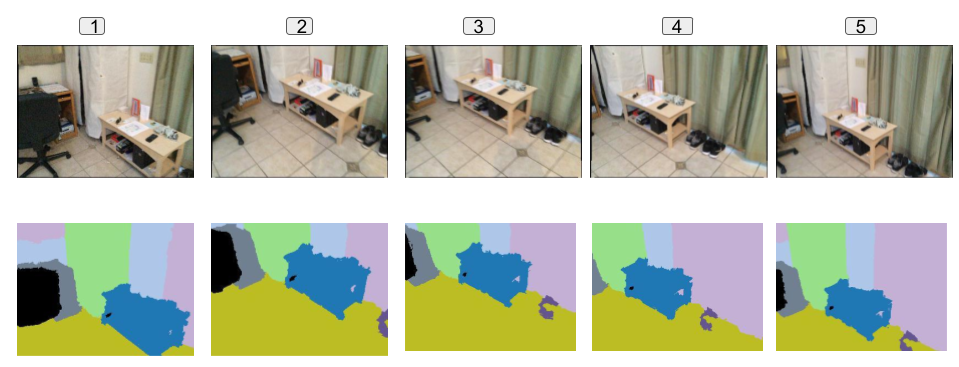
\includegraphics[width=17cm]{images/images_segm_scannet.png}
		\caption{Sample of Scannet dataset continuous frame rgb and semantic label. Courtesy of [91] }
		\label{fig:sample_rgb_seg_scannet}
	\end{figure}
        
	ScanNet is a video sequence dataset with 1513 scenes captured in 707 distinct spaces. The dataset contains a total of 2.5M RGB-D images. The dataset was initially designed for the task of indoor scenes 3D reconstruction, including 3D object classification, semantic voxel labeling, and CAD model retrieval [91], [92]. The dataset contains the details of the 3D camera poses, surface reconstruction, and instance-level semantic segmentation. One sample of the data is shown in the Fig \ref{fig:sample_pose_scannet}
	
	\begin{figure}
		\centering
		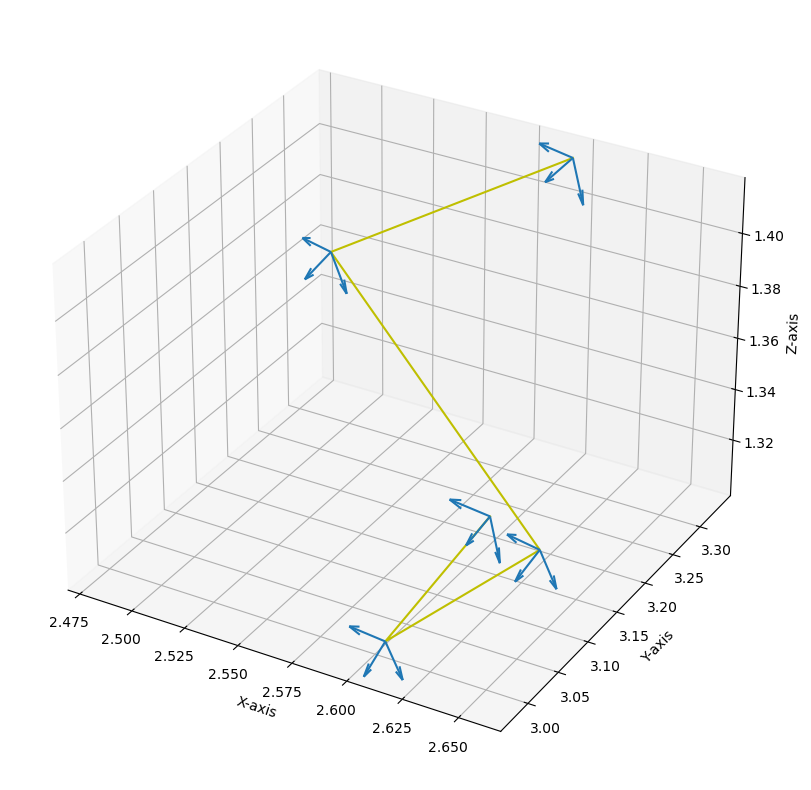
\includegraphics[width=11cm]{images/pose_viz_scannet.png}
		\caption{Sample of Scannet dataset pose. Each point represent the pose of the camera in 3D frame when a particular frame is captured. The representation shows how the camera is moving in the 3D world.}
		\label{fig:sample_pose_scannet}
	\end{figure}
	
	The 3D representation of the sample data is presented in the Fig \ref{fig:sample_pose_scannet}. There are 40 classes in the dataset, with different varieties under each category. The complete list of the classes is presented in Table \ref{table:Classes in scannet_1}, \ref{table:Classes in scannet_2}, and \ref{table:Classes in scannet_3}. Twenty users collect datasets at different countries' locations. Since the dataset is vast, a subset is taken for performing the experiments. Totally 186 video sequence data is taken for conducting the experiments. These video sequence data are further split into 149 sequences for training the model and 36 sequences for testing. The distribution of the scannet dataset labels is shown in figure \ref{fig:scannet_class_distribution}. There is a high number of pixels in the dataset belonging to the Wall, Other, Floor, and Chair categories. The dataset represents indoor scenes with different varieties. Hence experiments are conducted by combining the low pixel distribution class into single categories to balance the pixel distribution. 
	
	\begin{figure}
		\centering
		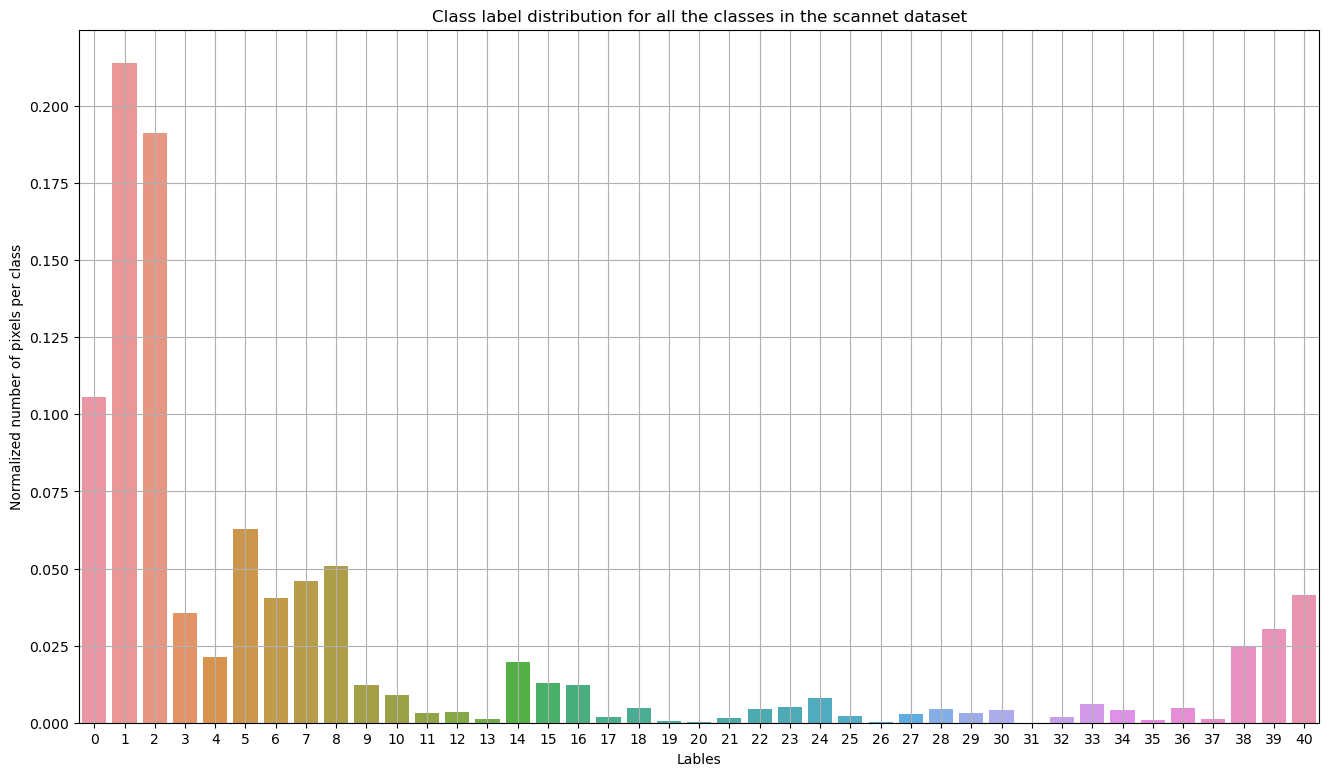
\includegraphics[width=11cm]{images/scannet_data_class_distribution.png}
		\caption{Scannet dataset class distribution. Horizontal axis represent the classes in Scannet dataset and vertical axis represent the normalized number of pixels per class. There are high number of pixels in entire data belonging to class 1 and class 2.}
		\label{fig:scannet_class_distribution}
	\end{figure}

  %  \subsection{Virtual KITTI 2 \ref{92_cabon2020virtual}}
    \subsection{Virtual KITTI 2 [93]}
    
	The virtual KITTI dataset is the first released to the public domain with driving applications. It is a synthetic dataset representing the simulation of the vehicle in different environmental conditions. And it is a cost-effective alternative to real-world data. Virtual KITTI 2 is the next-generation dataset with an improved photo-realistic and featured version of the original virtual KITTI dataset. The virtual KITTI 2 contains stereo camera views to expand the application areas. The dataset contains the exact five sequences clones with camera 0 representing the same dataset as virtual KITTI, and camera 1 is 0.5327m to its right. Each camera contains RGB, class segmentation, instance segmentation, depth, forward and backward optical flow, and forward and backward scene flow images. Each sequence contains camera parameters, vehicle color, pose, and bounding boxes. One sample from the sequence and corresponding pose representation in the 3D plane is shown in Fig \ref{fig:sample_scannet_vkitti_2} and \ref{fig:sample_pose_scannet_vkitti_2} respectively.
	 
	\begin{figure}
		\centering
		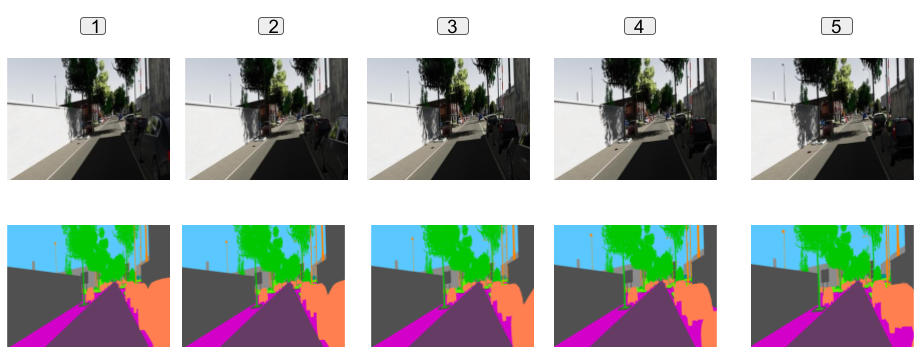
\includegraphics[width=14cm]{images/images_segm_vkitti.png}
		\caption{Sample of Virtual Kitti 2 dataset. Top row represent the continuous frame number followed by rgb and semantic labels. Courtesy of [93]}
		\label{fig:sample_scannet_vkitti_2}
	\end{figure}

	\begin{figure}
		\centering
		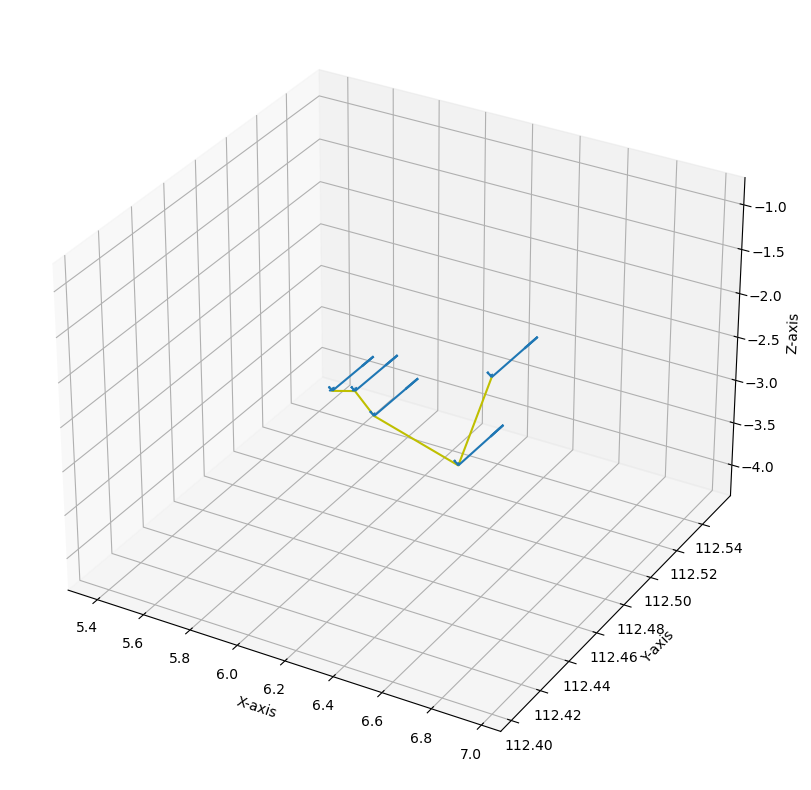
\includegraphics[width=14cm]{images/pose_viz_vkitti.png}
		\caption{Sample of Virtual Kitti 2 dataset pose. Each point represent the pose of the camera in 3D frame when a particular frame is captured. The representation shows how the camera is moving in the 3D world.}
		\label{fig:sample_pose_scannet_vkitti_2}
	\end{figure}
	
	\section{Data Collection and Preprocessing}
	
	After submitting the agreement terms, the RGB-D scannet dataset can be downloaded from the python script sent to the user from the dataset development group. The description and format of the dataset can be found on GitHub [94]. There are 1500 scans. Any specific scans, and file types,  can be downloaded. There is multiple information regarding a scan in a file. These files are further processed to color, label, pose, and depth data for each scan. More details are documented in the GitHub [95] repository. The raw RGB image is normalized before passing it into the model for quick convergence of learning. The input image is a 3-channel RGB data in .jpg format, the label is a single-channel image in .png format with 40 classes total, and the pose data is in text format. The pose data contains the rotation matrix and transnational vector inhomogeneous matrix format. The vkitti dataset is also in a similar format. However, there is a total of 15 classes in the vkitti dataset. The raw RGB image, label, and pose data are shown in Fig \ref{fig:scannet_vkitti}. 

	\begin{figure}
		\centering
		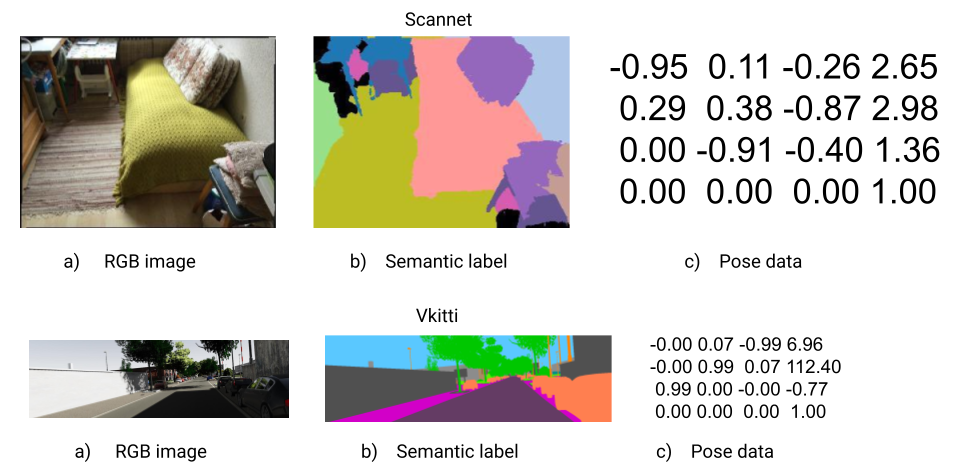
\includegraphics[width=14cm]{images/scannet_vkitti_data.png}
		\caption{RGB, Label and Pose sample of Scannet and Vkitti data}
		\label{fig:scannet_vkitti}
	\end{figure}	

	\begin{figure}
		\centering
		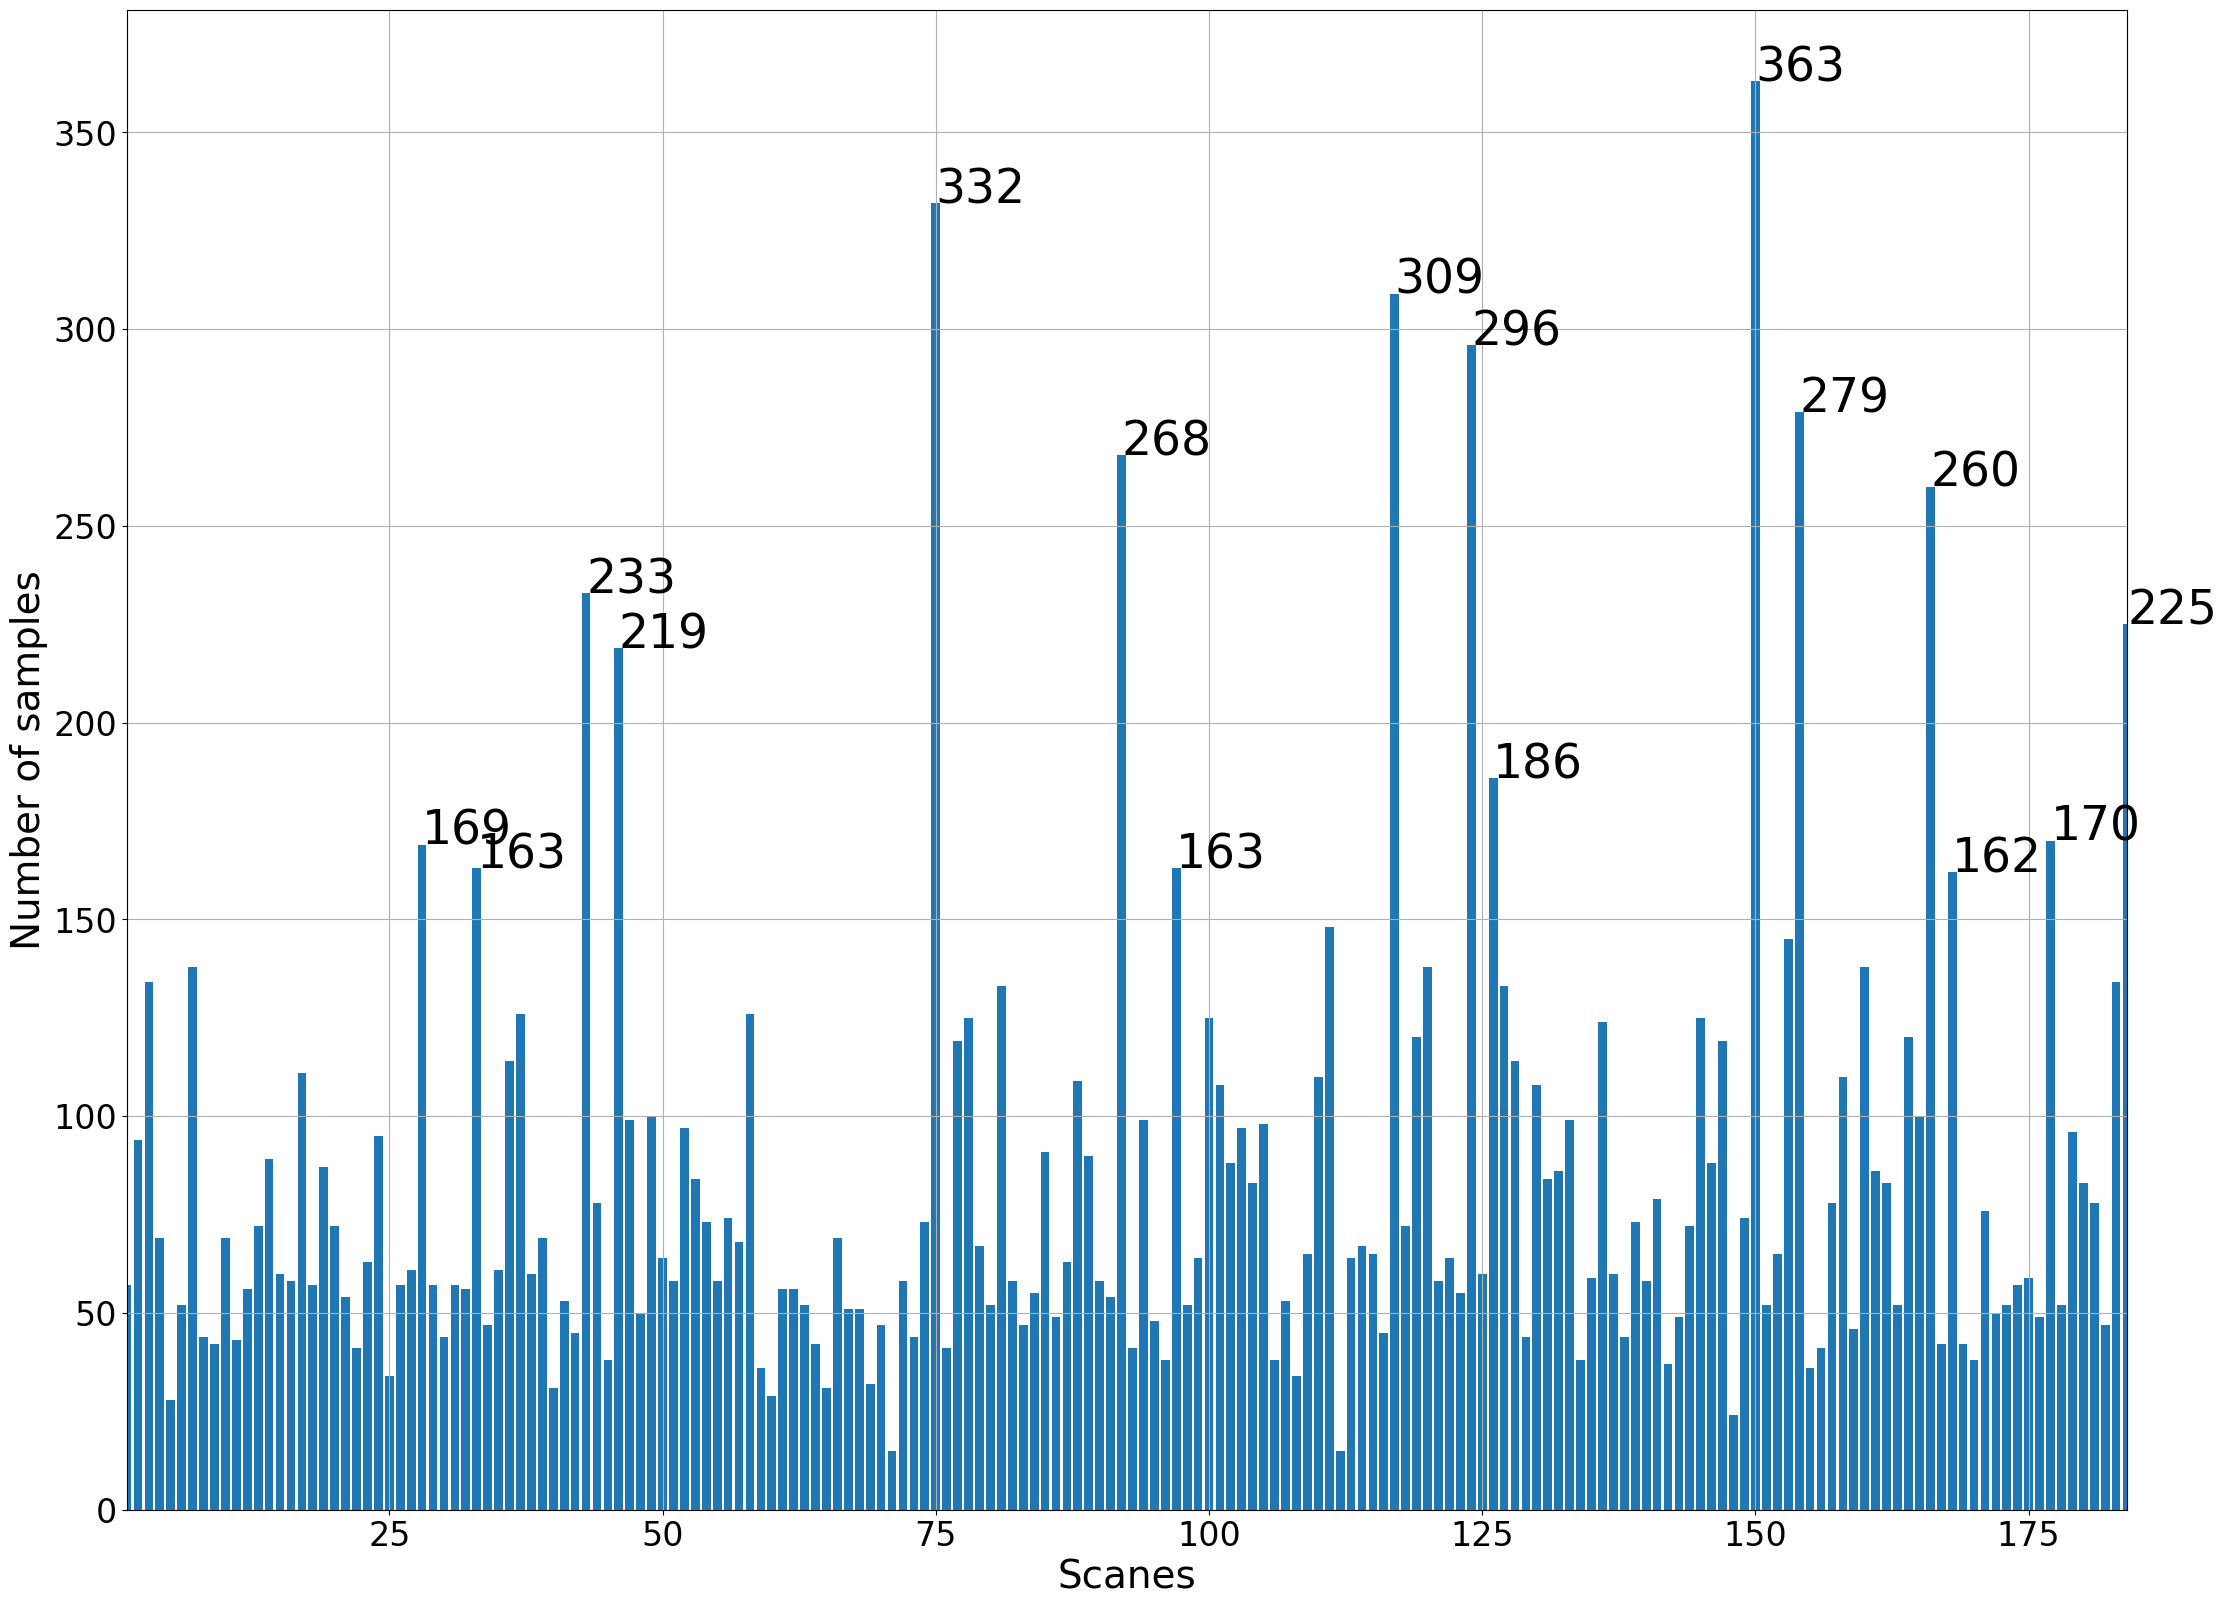
\includegraphics[width=14cm]{images/scannet_scanes_samples.png}
		\caption{Scannet data distribution. Horizontal axis represent the video sequence number and vertical axis represent the number of frames in each video sequence.}
		\label{fig:scannet_vkitti}
	\end{figure}

	\begin{figure}
		\centering
		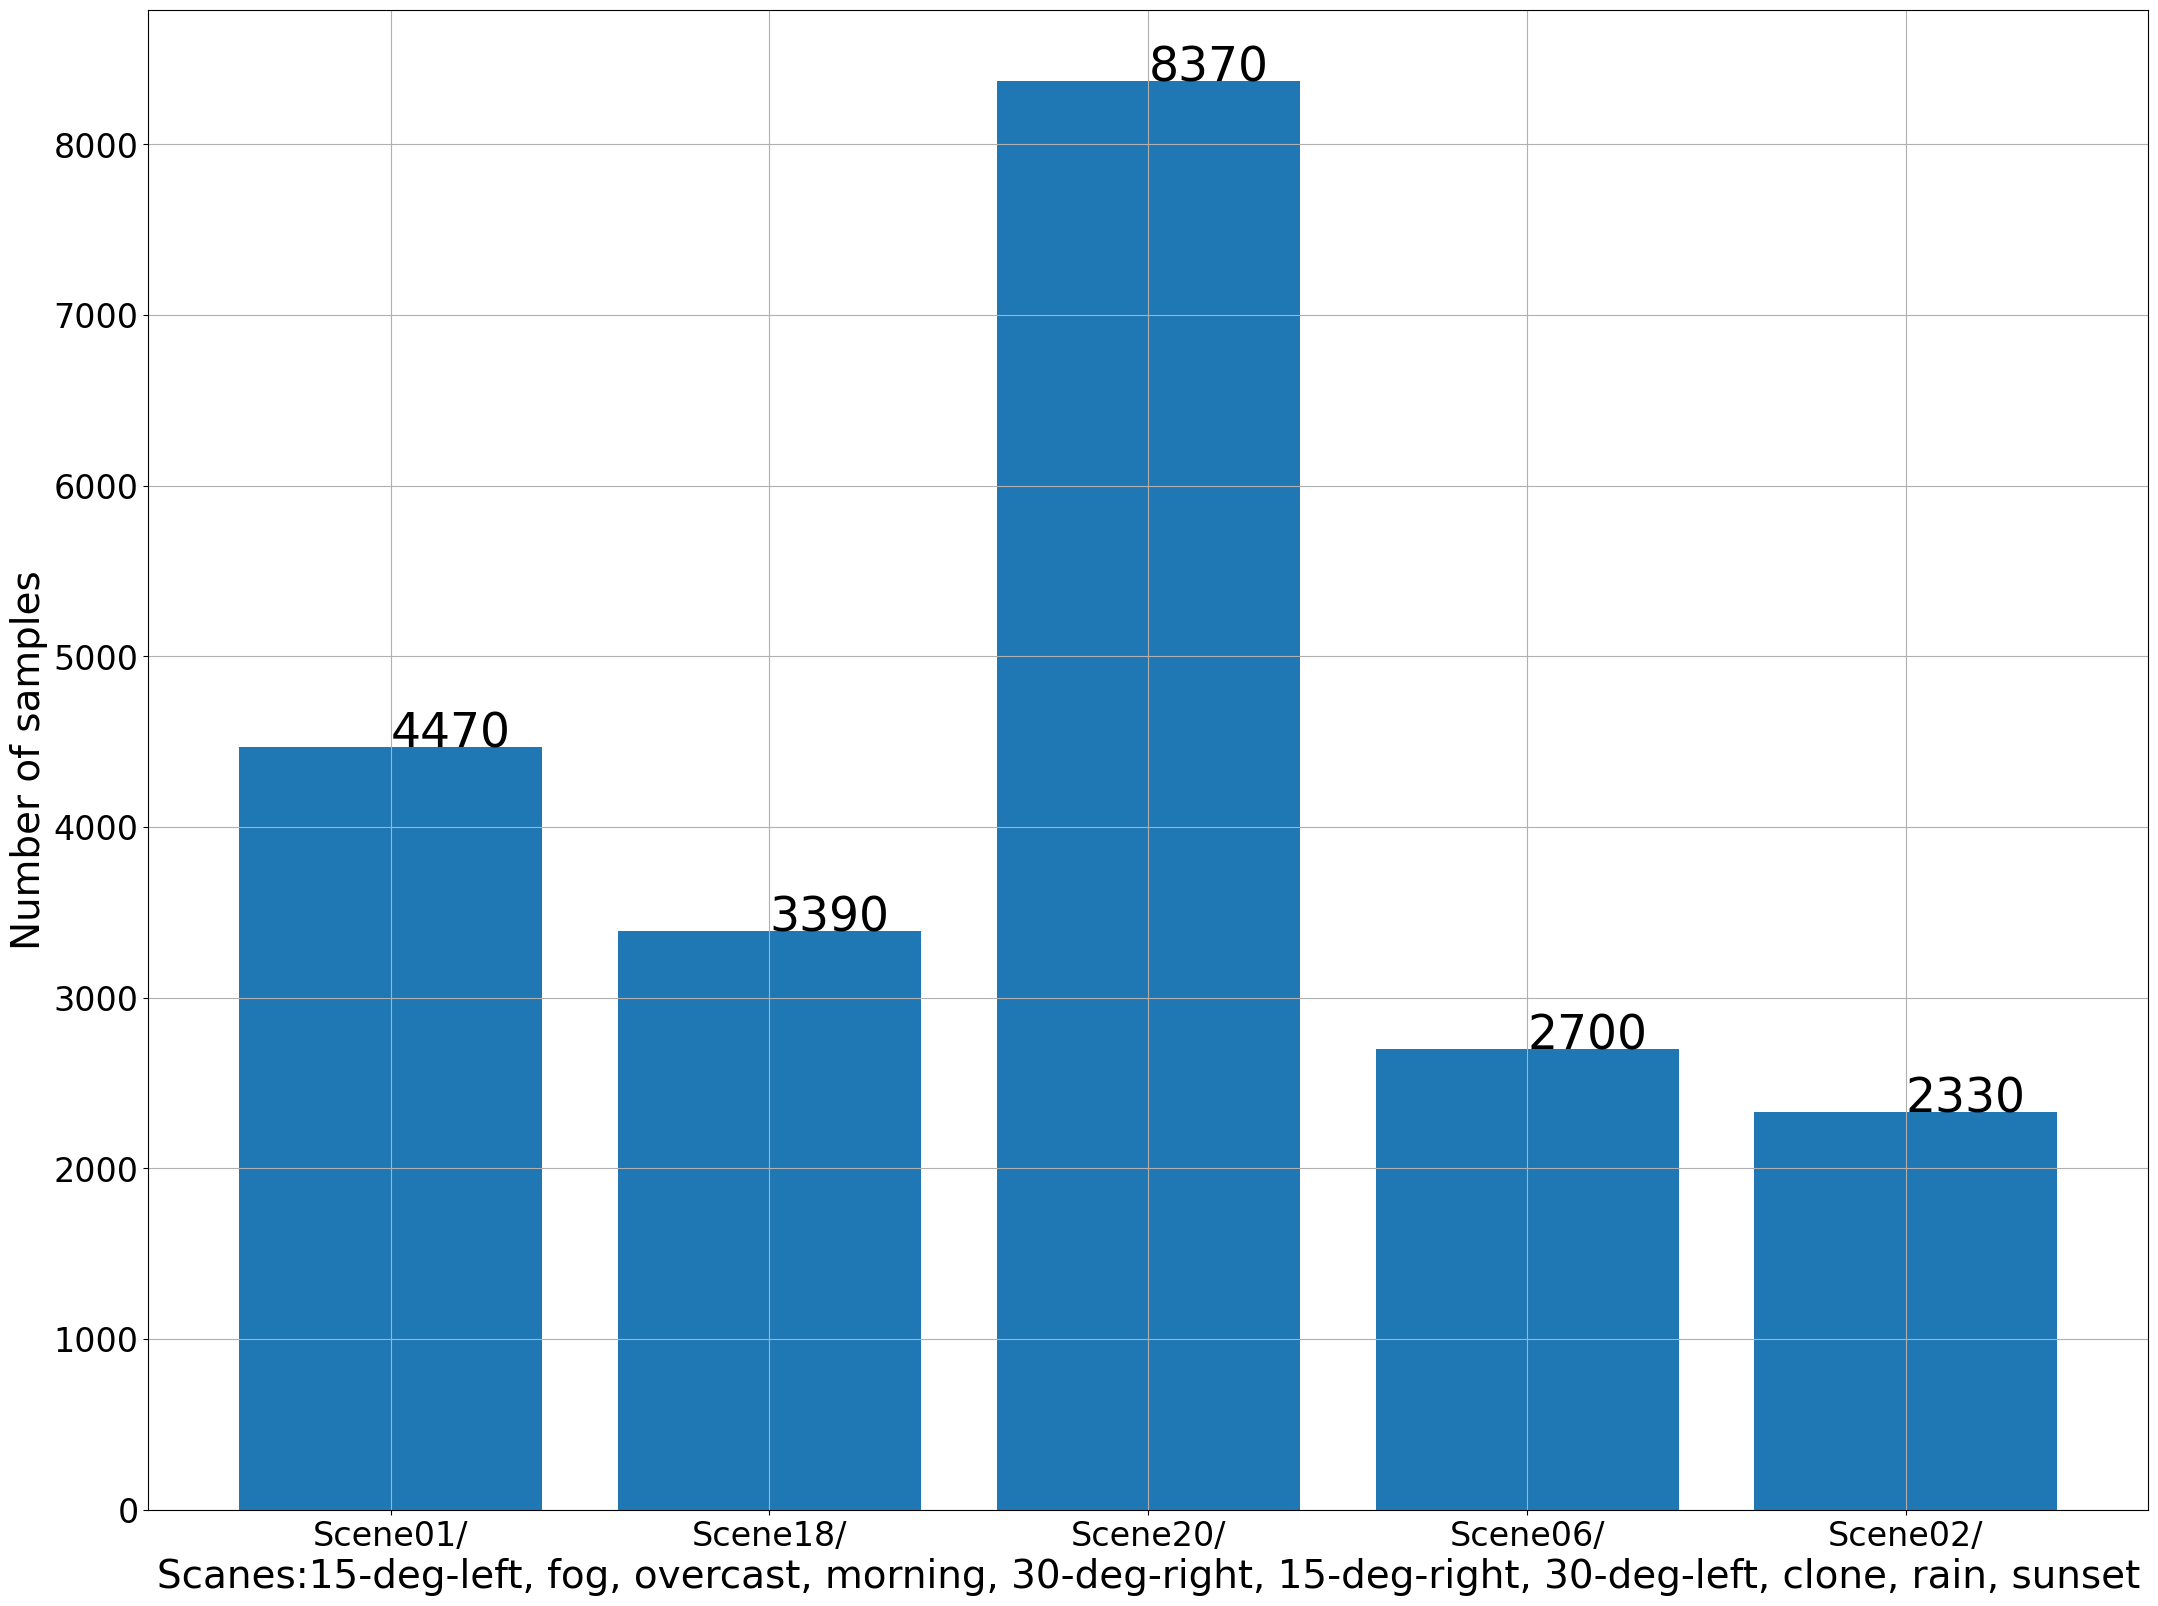
\includegraphics[width=14cm]{images/vkitti_scanes_samples.png}
		\caption{Vkitti data distribution. Horizontal axis represent the scenes and under each scene there is 15-deg-left, fog, overcast, morning, 30-deg-right, 15-deg-right, 30-deg-left, clone, rain and sunset categories.}
		\label{fig:scannet_vkitti}
	\end{figure}	
	
    \section{Experimental Design}
    
    The experiment aims to incorporate temporal fusion in the latent space to understand the impact of past frame information fusion in future frame segmentation prediction. The Unet model [7] perfectly suits this experiment. The unet model consists of an encoder and a decoder network with latent space encoding in between. Three types of experiments were conducted with the unet model. In the first type, the plain vanilla unet model is taken in the second type of experiment unet model with the gaussian process; the third type is the unet model with Long Short Term Memory (LSTM). In the last two experiments, the latent space encoding is subjected to temporal fusion by the gaussian process and LSTM.   
    
    \subsection{U-Net Vanilla Model}
    
	U-Net vanilla model is a simple semantic segmentation model with encoder-decoder architecture. The encoder is a contracting path, and the decoder is an expanding path. The input image is fed into the encoder, consisting of a convolutional neural net. The architecture consists of two 3x3 2d convolutional layers followed by a rectified linear unit (ReLU) and batchnorm2d with 2d downsampling Maxpool layer. At every step of the convolutional block, the number of out channels/ feature channels is doubled. From 64 features in the first convolutional block output to 1024 features at the downsampled fifth layer or the latent space encoding. The upsampling layer consists of a 2d convolution with a halved feature map at every step, followed by a concatenation of the corresponding feature map from the encoder path. The convolution2d consists of two 3x3 convolutions, each followed by a ReLU function. At the final layer of the decoder, a 2d convolutional layer was introduced to map the previous convolutional block output to the predicted class labels. There are 23 convolutional blocks in the entire network.    
	
	\begin{figure}
		\centering
		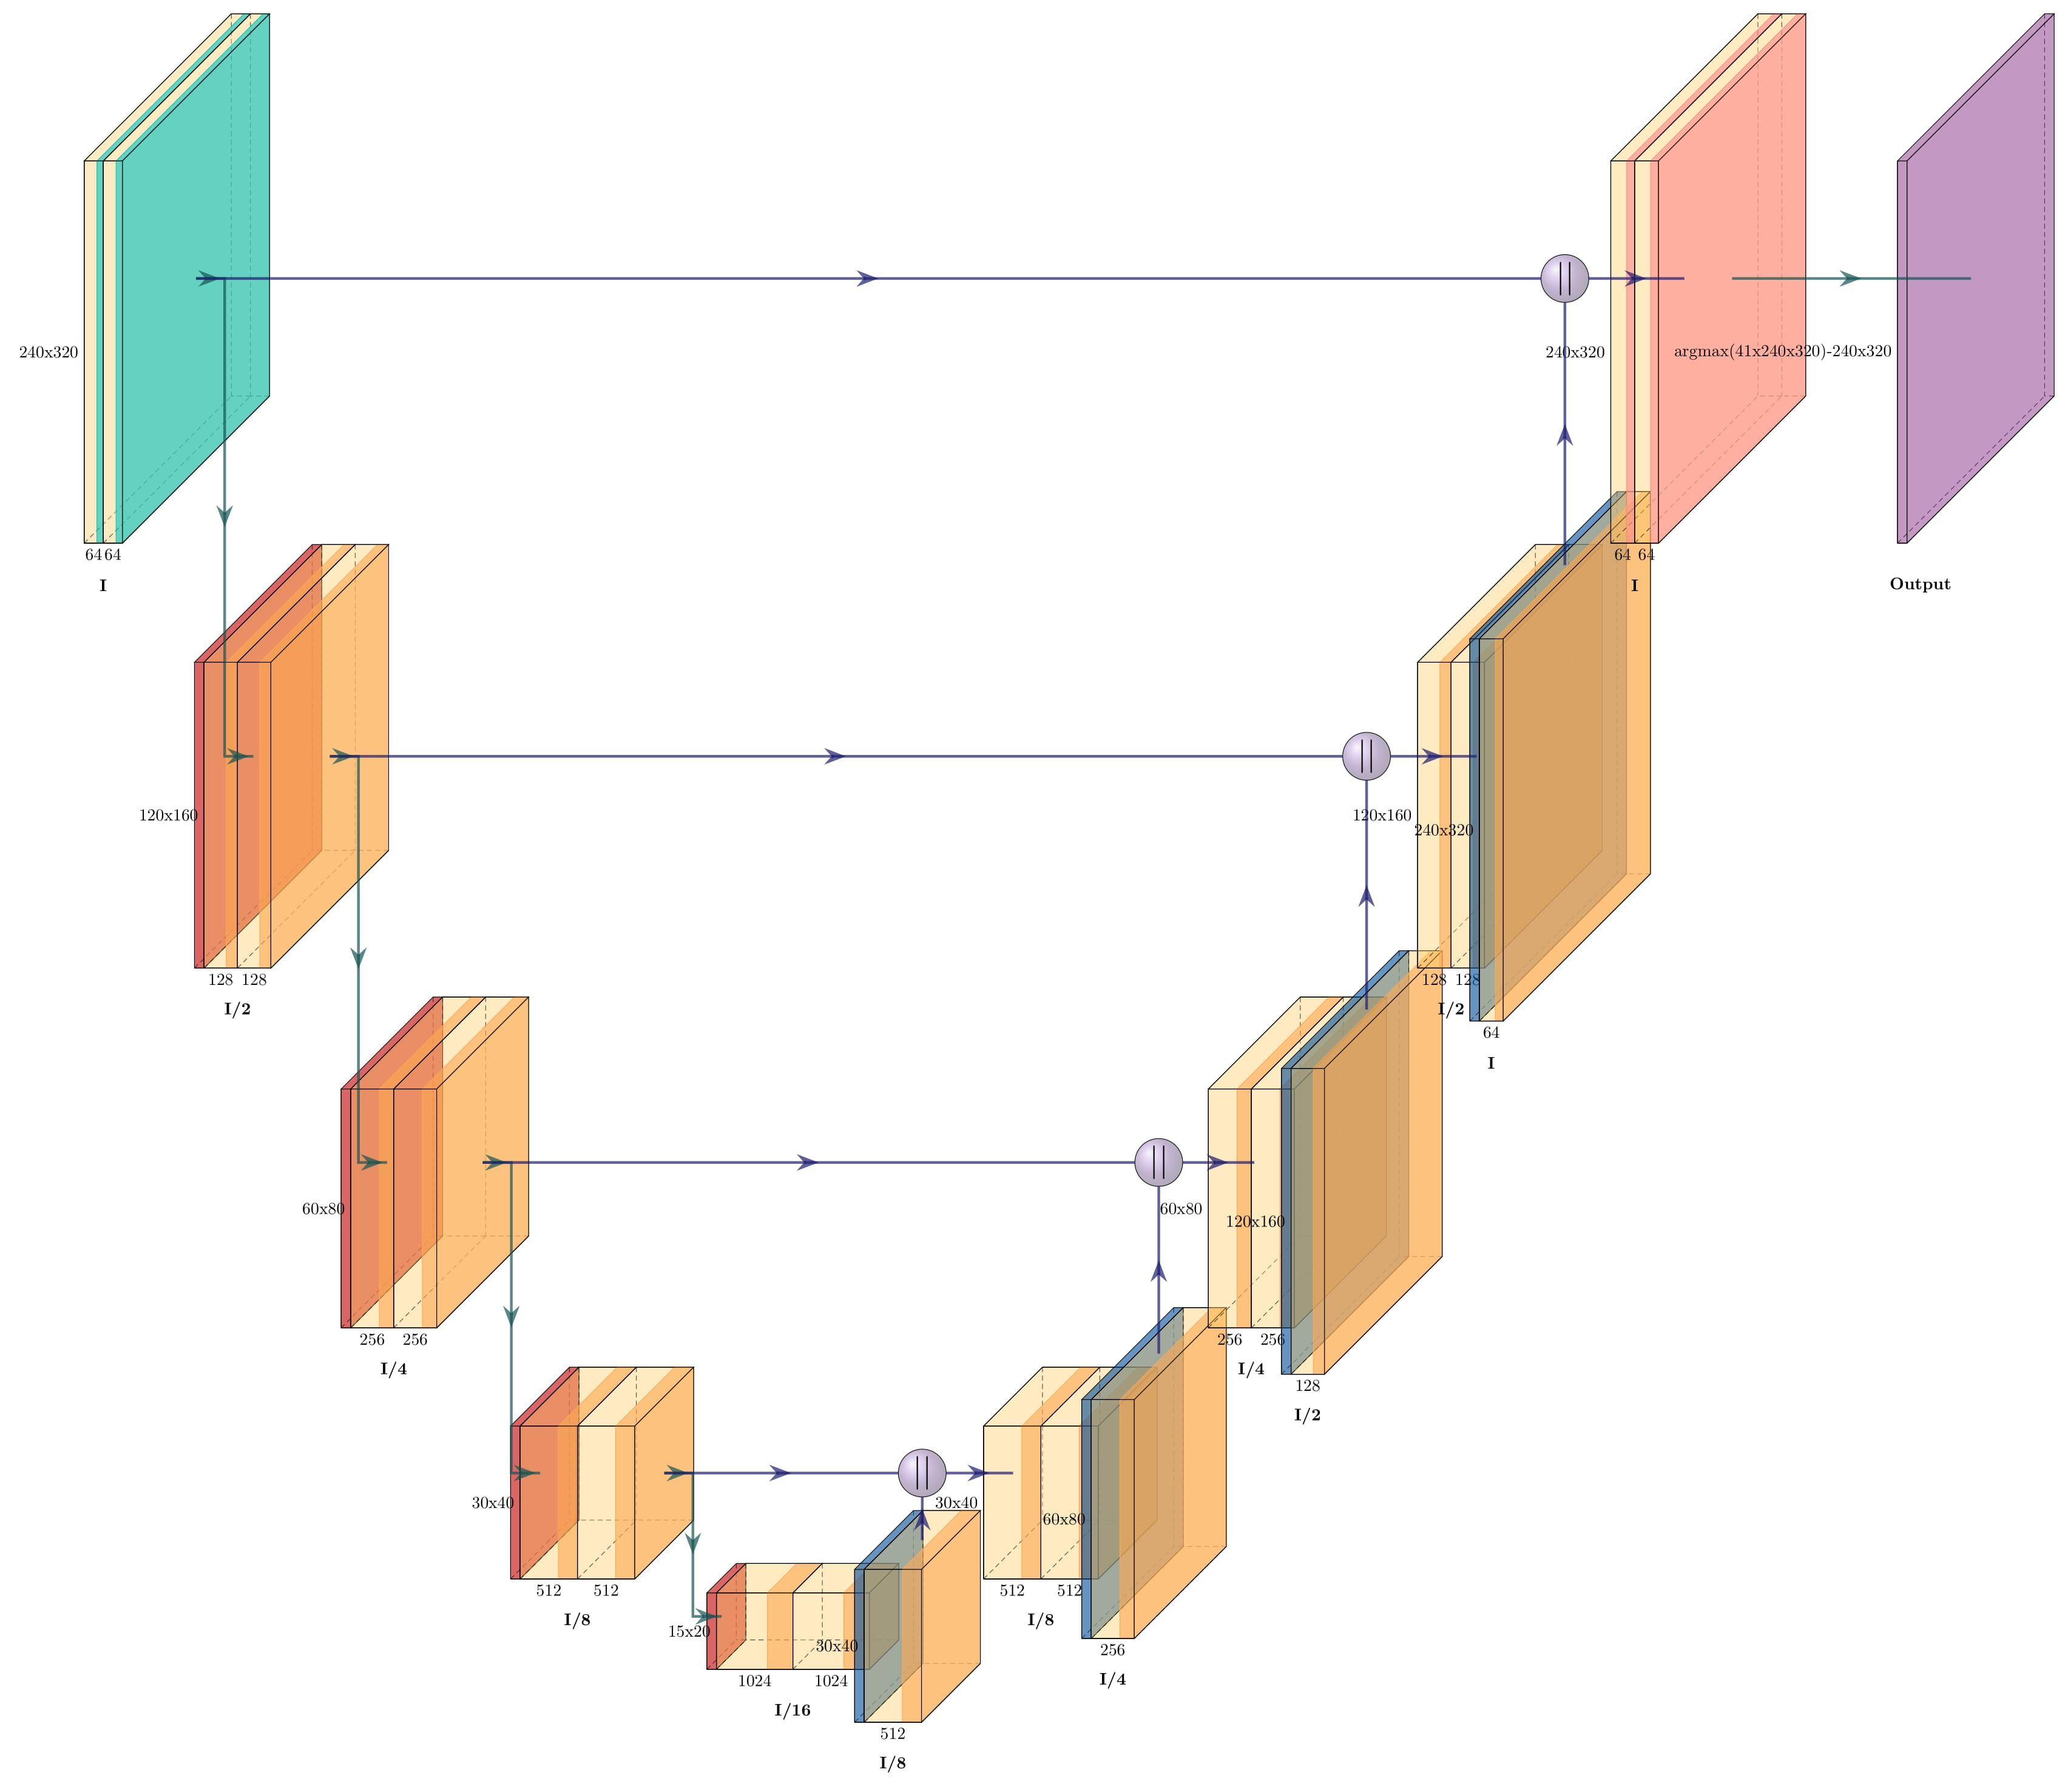
\includegraphics[width=14cm]{images/Unet.jpg}
		\caption{Unet model architecture. Generated with modification \href{https://github.com/HarisIqbal88/PlotNeuralNet}{PlotNeuralNet}}
		\label{fig:unet_model}
	\end{figure}
	
    \subsection{U-Net With Gaussian Process}
    
    In the second type of experiment, the latent space encoding of the U-Net model is taken and subjected to the gaussian process. The gaussian process ensures that the frames close to each other have similar latent space encodings. This is done by building the kernel of the gaussian process with a distance matrix. A probabilistic prior on the latent space accounts for the prior knowledge that poses very close have similar latent space encoding to the poses that are very far from each other. This information is encoded in the covariance matrix. The distance measured between the camera poses is calculated with a metric to define the closeness. The distance between the camera poses is calculated with the help of work by Yuxin Hou et al. [02] and Mazzotti et al. [97]. This measures the distance between the rigid body poses. The pose-distance measure between the two camera poses $P_i$, and $P_j$ is defined in equation \ref{eq:distance_matrix}. Where $t$ is the translation vector, $R$ is the rotational vector, $I$ is the identity matrix, and $tr()$ is the trace of the matrix.  
    
    \begin{equation}
     D[P_i, P_j] = \sqrt{{||t_i - t_j||}^2 + \frac{2}{3} tr(I - R_i^TR_j)}
     \label{eq:distance_matrix}    
    \end{equation}
	
	The covariance function is defined from this distance matrix $D[P_i, P_j]$. The covariance function is chosen from the Matern class [97] [98] in equation \ref{eq:covariance_matrix}.  
	
	\begin{equation}
		k(P,P') = \gamma^2(1+\frac{\sqrt{3}D[P,P']}{l}exp(-\frac{\sqrt{3}D[P,P']}{l}))
		\label{eq:covariance_matrix}
	\end{equation}
	The hyperparameter $\gamma^2$ and $l$ define the magnitude and length-scale of the processes. Independent GP priors to all values in $Z_i$, and the output of the encoder is assumed to be the noise corrupted version of the expected latent space encodings. The GP regression model is defined from this initialization settings and defined in the equation \ref{eq:encode_output} \ref{eq:gp} [02]. The architecture of the unet model with gaussian process is depicted in the Fig \ref{fig:unet_gp}. The encoder output is assumed to be noise corrupted hence the term $\epsilon_{j,i}$. 

	\begin{figure}
		\centering
		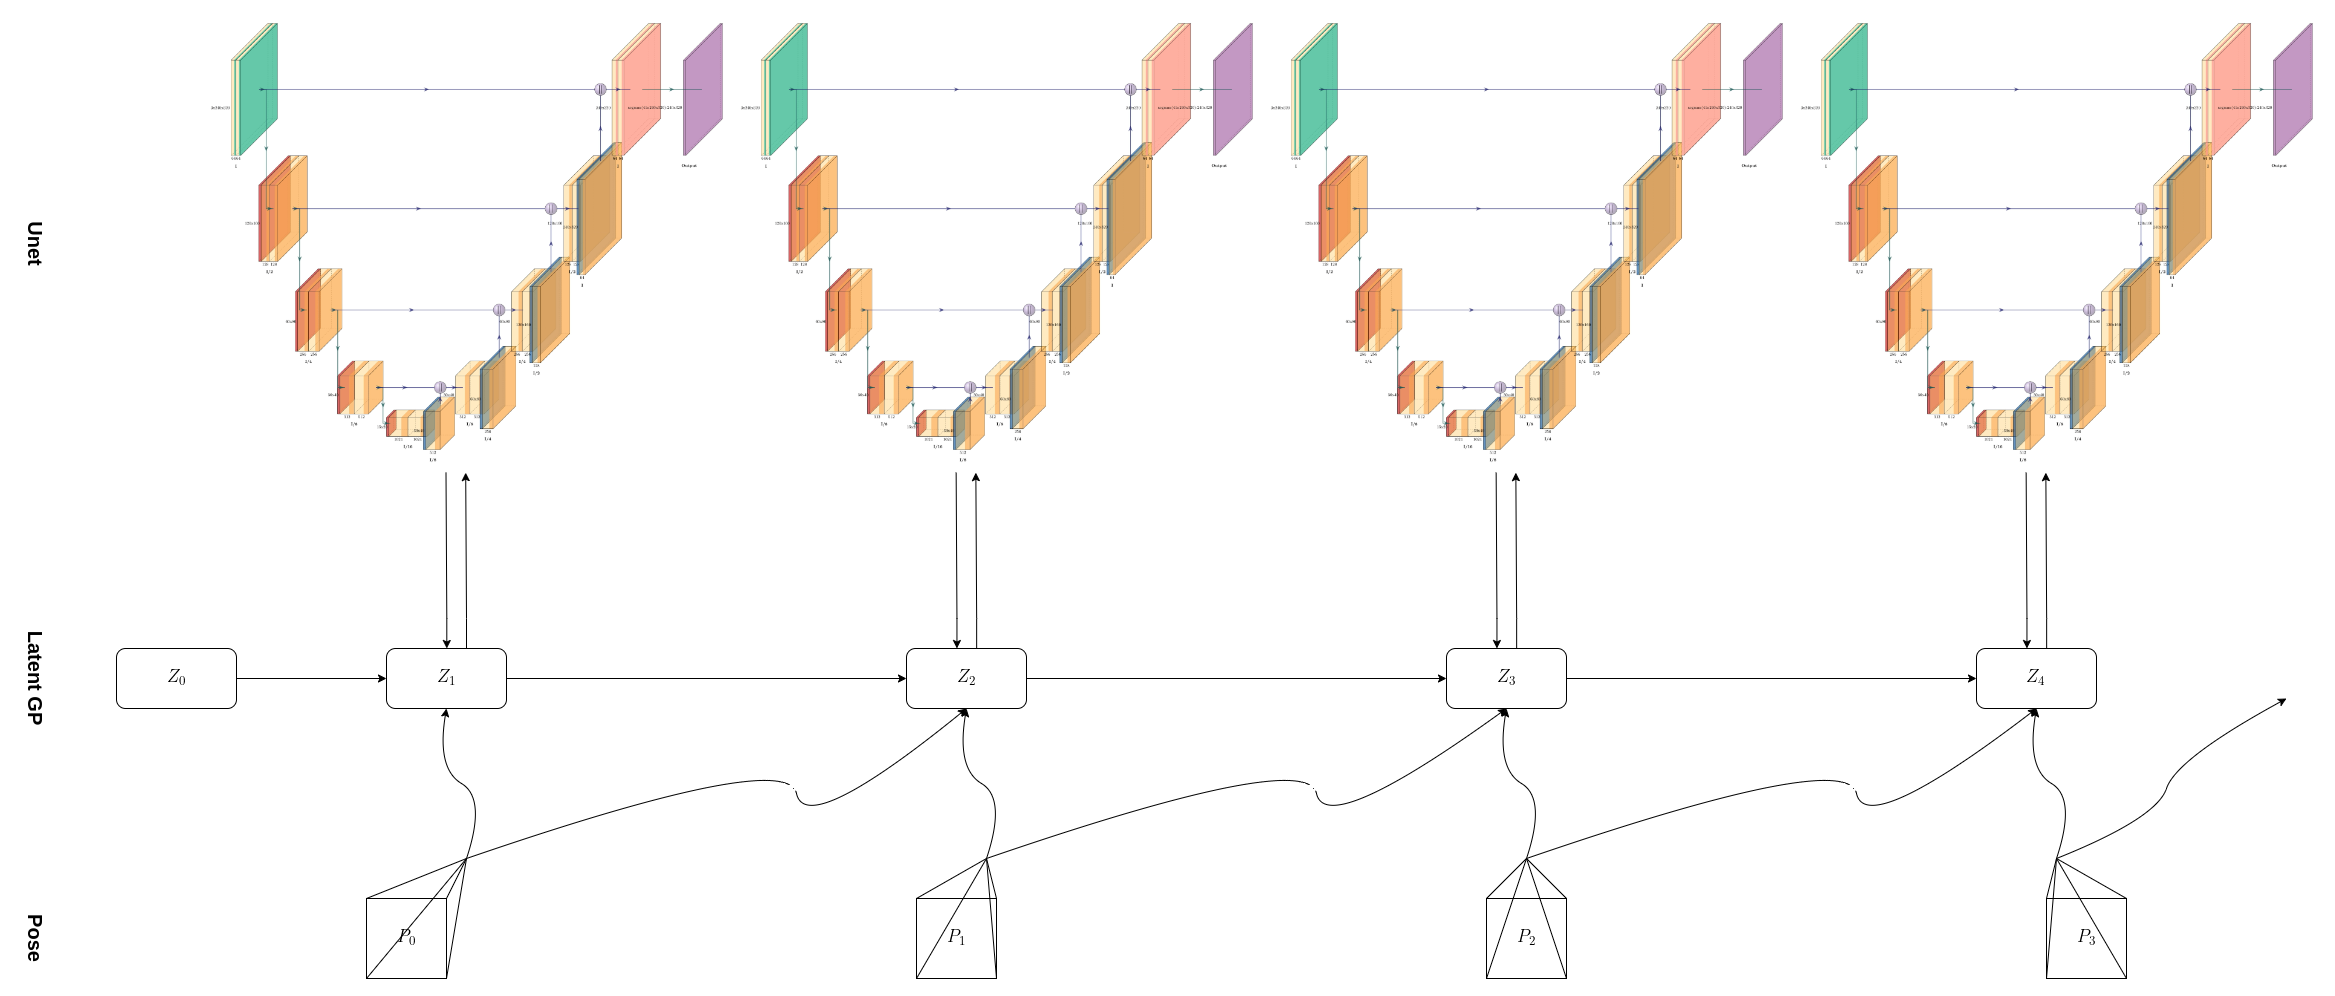
\includegraphics[width=14cm]{images/unet_gp.png}
		\caption{Unet model architecture with temporal fusion in latent space using Gaussian Process.The latent space encoding is propagated forward. During every computation the Gaussian Process takes latent space encoding, previous updated latent space and the current and previous pose to update the current latent space encoding. Generated with \href{https://app.diagrams.net/}{Diagrams.net}}
		\label{fig:unet_gp}
	\end{figure}

	\begin{equation}
		z_j(t) \sim GP(0, k(P[t], P[t']))
		\label{eq:gp}
	\end{equation}
	
	\begin{equation}
		EncoderOutput = z_j(t_i)+ \epsilon_{j,i}, \epsilon_{j,i} \sim  N(0, \sigma^2)
		\label{eq:encode_output}
	\end{equation}
    
    
    \subsection{U-Net with Long Short Term Memory (LSTM)}
    
    In the third type of experiment, the U-Net model is subjected to temporal fusion with the help of Long Short Term Memory (LSTM) by passing the latent space encoding onto the LSTM convolutional cell. The overlapping information in the consecutive frame data is passed onto the future frame prediction by incorporating the convolutional LSTM cell to improve performance and model the spatiotemporal relations compared to the vanilla model. The partial scene geometry information from the previous frame is used in the current step frame prediction. A hidden state propagation approach from the LSTM method is used to pass the latent space information. The adaption of temporal fusion with LSTM is inspired by the work of Arda Düzçeker et al. [13]. The author introduced a convolutional LSTM cell in the latent space to learn the shared information between the frames to predict the depth of objects in video sequence data. The convolutional LSTM cell is inspired from [99]. The original LSTM version is explained in the article [100]. The hidden state $H$ and cell state $C$ are initialized to a value. Let $X$ denote the output of the bottleneck encoder network, then the logic to compute the hidden state and current state can be calculated as below (Courtesy of [13])
    
    \begin{equation}
    	i_t = \sigma(w_{xi}*X_t+w_{hi}*H_{t-1})
    	\label{eq:it}
    \end{equation}
    \begin{equation}
		f_t = \sigma(w_{xf}*X_t+w_{hf}*H_{t-1})
		\label{eq:ft}
	\end{equation}    
    \begin{equation}
	 	o_t = \sigma(w_{xo}*X_t+w_{ho}*H_{t-1})
	 	\label{eq:ot}
 	\end{equation}   
    \begin{equation}
	    g_t = ELU(layernorm(w_{xg}*X_t+w_{hg}*H_{t-1}))
	    \label{eq:gt}
    \end{equation}
    \begin{equation}
	    C_t = layernorm(f_t \bigodot C_{t-1} +i_t \bigodot g_t)
	    \label{eq:Ct}
    \end{equation}
    \begin{equation}
	    H_t = o_t \bigodot ELU(C_t)
	    \label{eq:Ht}
    \end{equation}
    
    Where $*$ denotes the convolution, $\bigodot$ is the Hadamard product, $\sigma$ is the sigmoid activation function, and $w$ is convolution filter weights. Fig \ref{fig:unet_lstm} presents the exact pictorial representation. Each frame of the sequence video is passed onto the bottleneck U-net model in order, and prediction is made for individual frames. The output from the encoder network is passed through the LSTM cell. The output from the first LSTM cell act as the input to the subsequent LSTM cell computation; thereby, it carries the learned information forward from one frame computation to the following frame computation.   
    
	\begin{figure}
		\centering
		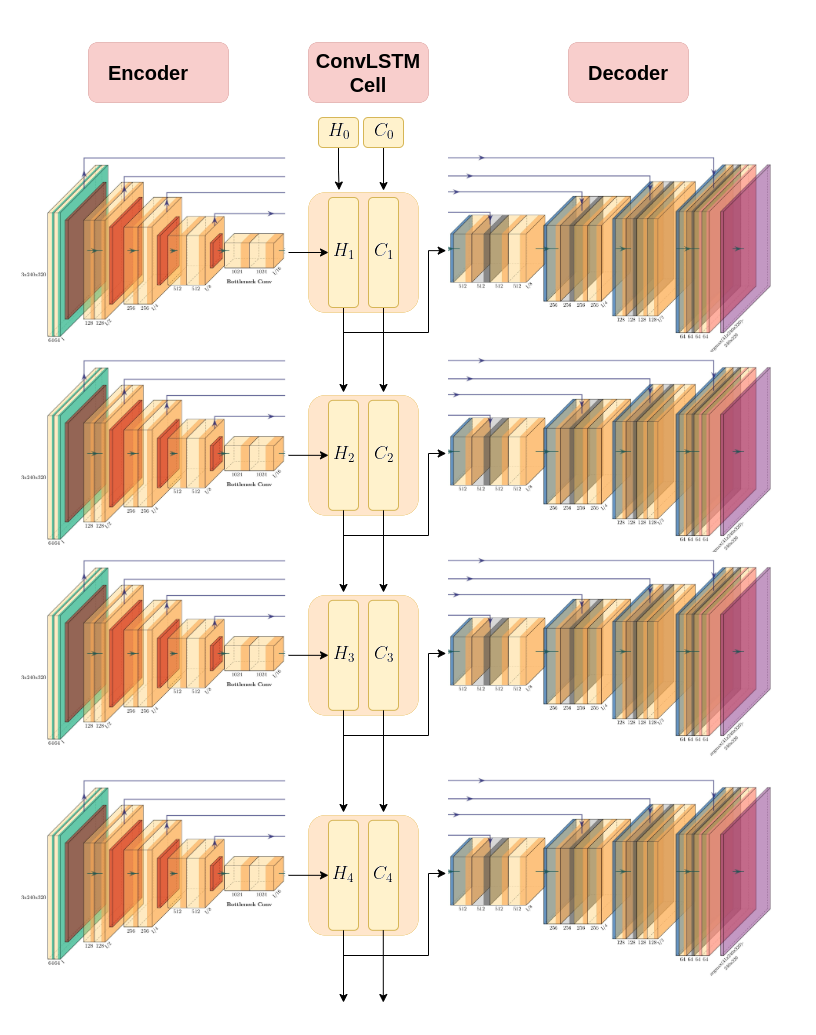
\includegraphics[width=14cm]{images/unet_lstm.png}
		\caption{Unet model architecture with temporal fusion in latent space using the ConvLSTM cell. At every frames semantic label computation the previous convolutional LSTM cell hidden and cell state are passed to the current cell computation. Thereby modeling the temporal dependency in the consecutive frames. Generated with \href{https://app.diagrams.net/}{Diagrams.net}}
		\label{fig:unet_lstm}
	\end{figure}     
        
    \section{Training and Evaluation Pipeline}
    
    Datasets are split into training and evaluation sets. During the training phase, the image, label, and pose paths are added to a list and then passed onto the data loader. The image data is read and normalized. The experiment is conducted with a different number of classes by merging the classes. This is done in the label processing stage. A model is initialized with different parameter settings. The processed image, label, and pose data are passed onto the initialized model. A loss criterion is defined to compute the losses. Loss is computed from the ground truth value and the model prediction. Backpropagation from the loss is calculated, followed by the optimization step. In the final stage, the loss and model are saved. The data loader loads data in batches. The process is repeated until all the data in the data loader iterate through the entire data once. The entire process is repeated for a different number of epochs. Model performance is monitored during each epoch run and stopped once the loss reaches a small value and the model fits the training data. 

	The evaluation dataset path is stored in the list during the evaluation process. The individual list contains Image, Label, and Pose path information. Since the dataset is a continuous sequence data, the path of the data stored in the list is in order. In most cases, there is overlapping information between the consecutive frames. In the evaluation, datasets are passed onto the data loader. Images are normalized from this data loader, and labels are processed per the experiment's requirement. Pose information is in text format. The text data is read, passed to a list, and returned by the data loader. The trained model is loaded, and the processed data from the data loader is passed onto the model. The predicted output from the model is evaluated against the evaluation metric, and the results are saved.      
    
    
   	\begin{figure}
    	\centering
    	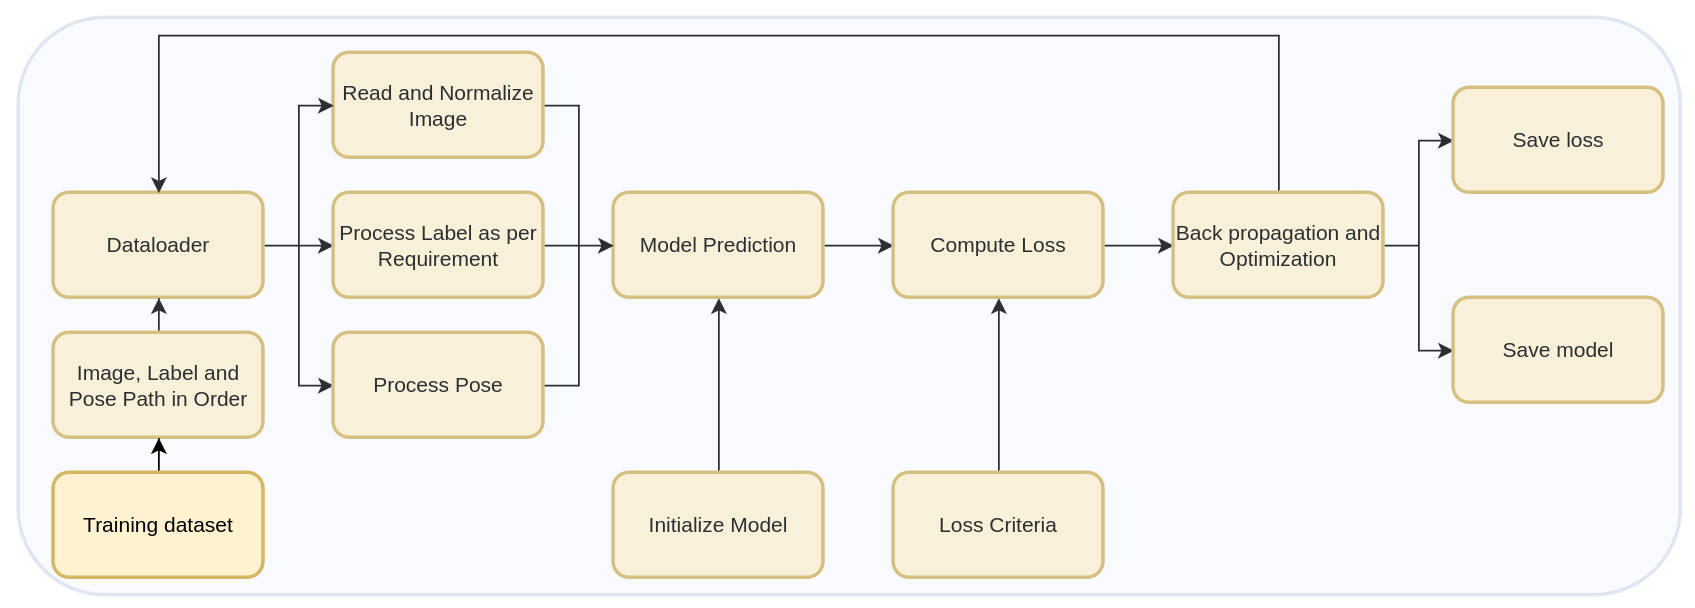
\includegraphics[width=14cm]{images/training.png}
    	\caption{Training pipeline. Generated with \href{https://app.diagrams.net/}{Diagrams.net}}
    	\label{fig:unet_training}
    \end{figure}

	\begin{figure}
		\centering
		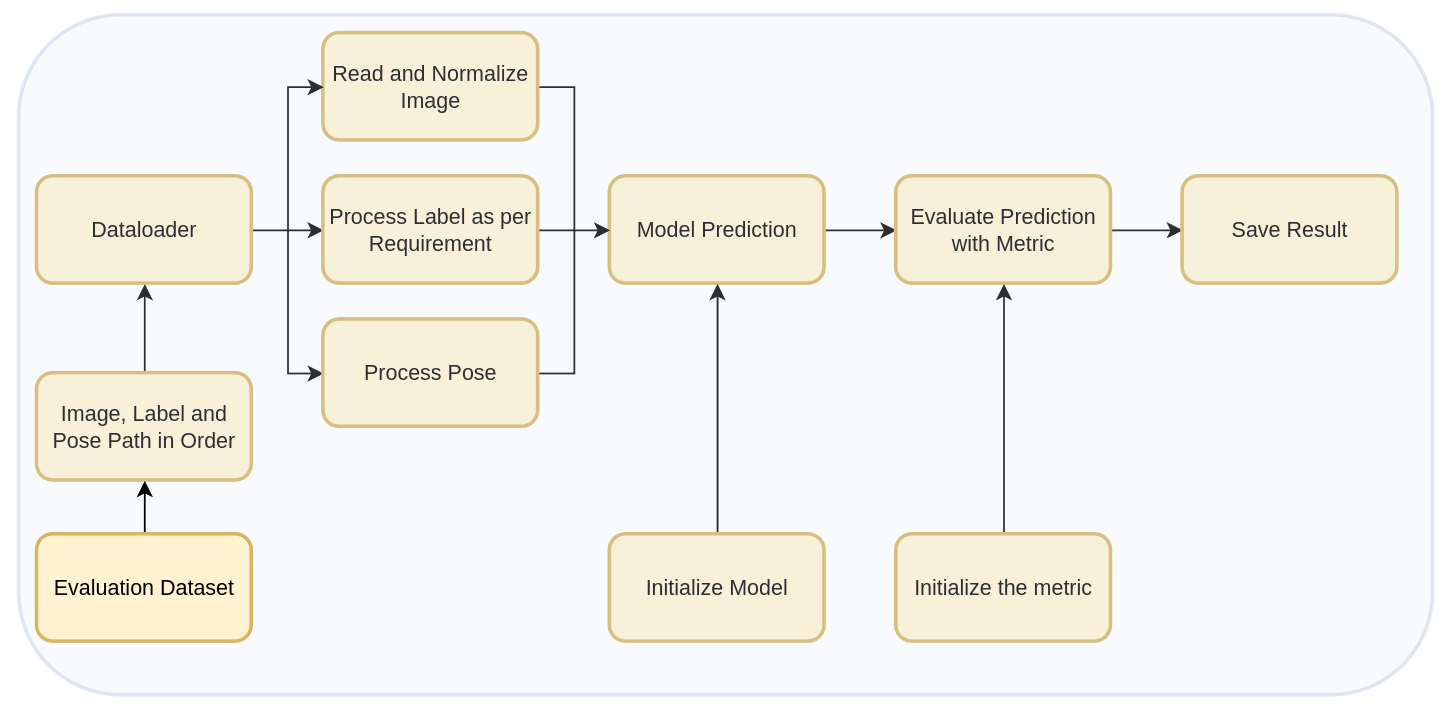
\includegraphics[width=14cm]{images/evaluation.png}
		\caption{Evaluation pipeline. Generated with \href{https://app.diagrams.net/}{Diagrams.net}}
		\label{fig:unet_evaluation}
	\end{figure}

	\begin{figure}
		\centering
		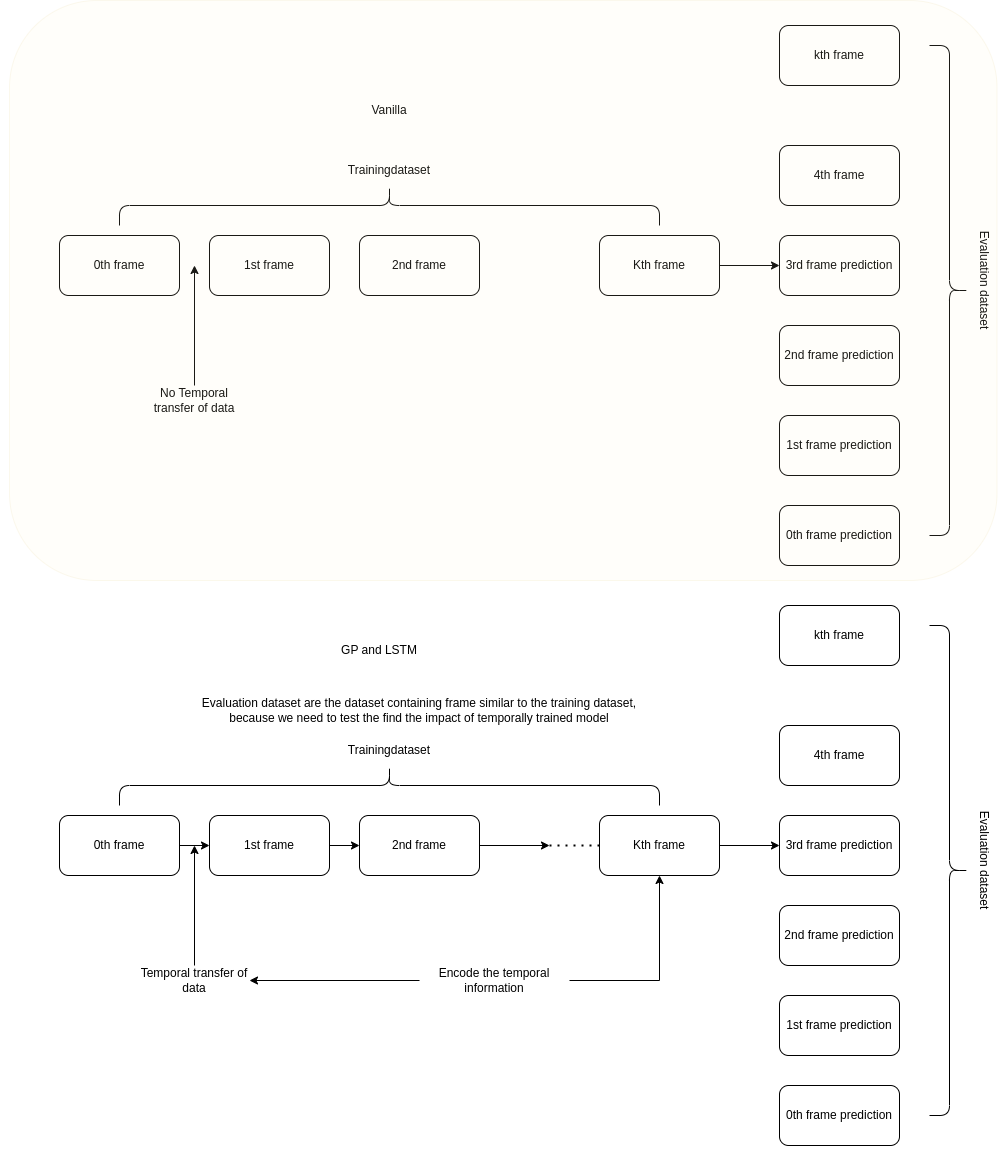
\includegraphics[width=14cm]{images/training_and_evaluation.png}
		\caption{Pictorial representation of training and evaluation procedure. The picture represent the how the training and evaluation is conducted with and without the temporal fusion. In the Vanilla network the model is trained on individual frames without temporal fusion and in the GP and LSTM model temporal data is propagated from one frame to another. Generated with \href{https://app.diagrams.net/}{Diagrams.net}}
		\label{fig:unet_evaluation}
	\end{figure}

    \section{Hardware Configuration}
    
    Training of the models is carried out in different sources. The workstation used to train and evaluate the models involve NVIDIA GeForce RTX 3070 Laptop GPU, 8192 MB, Tesla T4, 12680 MB, Google Colab, and Nvidia Tesla V100 PCIe GPU with 5120 Cuda cores, and 640 Tensor cores, 16 GB HBM2 memory University cluster. 
    
\end{document}
